\chapter{Evaluation}

This chapter covers the evaluation of the final product, the process model and what the team learned in this course.

\section{Problems and Difficulties}

	The first problem the group encountered, was to not use incompatible licenses. This was quite hard because much is licensed as GPL 1 or 2 and are not compatible with Apache 2. \\

	The second problem was the decision to write the protocol or use a middleware on a computer.

	The last problem was to get the protocol to work.

\subsection{Protocol}
There were several difficulties related to programming the Arduino. There were few existing solutions for programming it in general, and none for Android or Java. The official implementation was available in C, but in the incompatible GPL license.\\

The existence of certain programs written in Java with the purpose of programming Arduinos,
led the group into assuming one of these could be utilized, as the license was compatible. When the time came to make use of it, it was discovered to internally use AVRDUDE as well - an embedded version was available for several platforms.\\

This realization came somewhat late in the process, see Iteration 4 in the appendix on page \pageref{Iteration4}. Following this and the emergency meeting with the customer, it was decided to implement the protocol for programming Arduinos. Unfortunately, the documentation for these were a bit confusing; the most detailed and professional protocol document turned out to describe version 2 of the protocol\cite{AVR068}, which was incompatible with the bootloader installed on the Arduino by default (Optiboot v4.4 on Arduino Uno). This was also the version that was partially implemented before the protocol differences and lack of backwards compatibility was discovered.\\

The incompatibility could have been discovered earlier, but testing of the protocol had to be postponed due to a lack of available working serial communication libraries for PC's compatible with the Arduino Uno USB interface, so a simple Android I/O app was added for testing purposes. Even then, the reason for the failure to communicate with the Arduino was hard to pin down, until a second Arduino was wired up to echo back the information the pair received.\\

Changing the bootloader to utilize version 2 of the protocol could not be done due to it being licensed under GPL. Some attempts were made at finding compiled bootloaders for the Uno, but did not bear fruit. Attempts at compiling bootloaders using version 2 for the chip failed due to unresolved dependencies in the bootloader projects discovered, like the Stk-Boot\cite{Stk-Boot} and uOS-Embedded\cite{uOS-Embedded}.

The solution, then, was to implement version 2 of the protocol, and write off most of the protocol work as waste (a bit less than a week); some of it could be reused despite the protocols being radically different, however. The second version of the protocol has a standardized message format with checksums and static tokens inside the messages to aid in error discovery; this would have been beneficial for communicating over Bluetooth.\\

It was known that Optiboot didn't make use of all the commands specified in the protocol document AVR061\cite{AVR061}, but documentation on which commands were required or superfluous was lackluster. Since it would simply report that everything is fine when encountering such a command, discovering which were implemented or not had to be done by trial and error or investigating the source (which is designed to be very compact, to fit in the 512kB threshold).\\

Communicating with the Arduino proved fairly straight forward, but dealing with false positives was an issue.
The Arduino would report that writing took place successfully, but writing would occur only in partial sections of the memory areas requested, for example. The only way erroneous writing could be discovered, was to read afterwards to verify the contents (or observe the Arduino not starting run the code it was supposedly programmed with).\\

These issues prolonged the development of the system by a considerable amount, and had a major impact on the project. Some
of these could have been avoided by more careful initial investigation, while others would not have been apparent prior to implementing the protocol.

\section{Interaction with the customer}

	The communication with the customer was great. A regular meeting was held every Friday, and the customer had an insight to the projects repositories, this way the customer always knew what was going on. 



\section{Group interaction}
	The group decided upon regular meetings three days a week, where people sat down and worked together, discussed issues and progress. It was said that during a larger course like this, every member should work approximately 20 hours every week, thus this was quickly agreed upon. Apart from the regular meetings, the members were able to work at flexible hours within the iterations.
	In Table ~\ref{table:workhours} the total workhours for the group on every iteration is listed.

	\begin{table}[H]
	\caption{Iterations and time spent}
	\centering
	\label{table:workhours}
	\begin{tabular}{|l|l|}
		\hline
			{\bf Iteration} & {\bf Hours}\\
		\hline
			Iteration 1 (Week 6-7) & 186 hours\\
		\hline
			Iteration 2 (Week 8-9) & 257 hours\\
		\hline
			Iteration 3 (Week 10-11) & 233 hours\\
		\hline
			Iteration 4 (Week 12-13) & 129 hours\\
		\hline
			Iteration 5 (Week 14-15) & 195 hours\\
		\hline
			Iteration 6 (Week 16-17) & 220 hours\\
		\hline
			Iteration 7 (Week 18-19) & 263 hours\\
		\hline
	\end{tabular}
	\end{table}

	An associated chart diagram of the workhours are shown in Figure ~\ref{fig:workhours}

	\begin{figure}[H]
	\centering
	\captionof{figure}{Workhours in each iteration}
	\label{fig:workhours}
	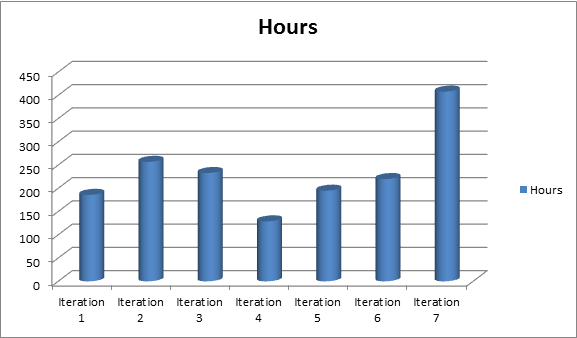
\includegraphics[scale=0.8]{images/workhours_chart2.png}
	\end{figure}

	\section{Process}
	The overall process has been going well. The group have learned to document issues and tasks on the way. This made the process flow steady forward and made it clear and organized. Every member always knew what to do when he or her checked the issue list on Git.

	The communication in the group was also good, the group worked together almost every day and had a group meeting every week. The group could also contact each other via Skype, phone and email.

	Mistakes were made however. During the first few weeks of the project, much of the focus was on the android application. Be it design or actual coding for android. The general consensus was that the android application would take approximately the same amount of time as the protocol for transferring files from the android device to the arduino device. This was on the background that a java implementation of the STK500 protocol existed, but poor research was done and it proved to be unusable.

	\section{The System}
	The $\mu$C Software Store application is almost ready to use. A few changes is still needed to be implemented before it can enter the market. First and foremost is the creation of proper applications within the store. The following is a short analysis of the system by the deadline of the project.\\



		\subsection{Protocol}
			- Used more time than expected\\
			- Change from STK500v2 to STK500v1\\
			- Had major impact on the project\\
			- Not enough research on the protocol in the beginning of the project\\

		\subsection{Bluetooth connection}

		\subsection{Store application}

	\section{Conclusion}
    The project was successful and the most important requirements including the biggest problem (the protocol) was met. The frequent group meetings, customer meetings and the organized structure of issues, turned out to be a great achievement. \\

    	\subsection{Requirements met}

			- GUI\\
			- Bluetooth connection\\
			- QR-code and SerialInput\\
			- Retain a reliable connection to the connected device\\
			- Remember the device from last time and try to reconnect\\

		\subsection{Requirement not met}
			- Sync Adapter\\
			- External database\\
			- Filter application by compatibility\\
